\documentclass[aspectratio=169,11pt]{beamer}

% ===== Theme & Colors =====
\usetheme{default}
\usecolortheme{default}

% Custom colors
\definecolor{primary}{RGB}{33, 37, 41}
\definecolor{secondary}{RGB}{108, 117, 125}
\definecolor{accent}{RGB}{0, 123, 255}
\definecolor{success}{RGB}{40, 167, 69}
\definecolor{warning}{RGB}{255, 193, 7}
\definecolor{danger}{RGB}{220, 53, 69}
\definecolor{light}{RGB}{248, 249, 250}

% Apply colors
\setbeamercolor{frametitle}{fg=primary}
\setbeamercolor{title}{fg=primary}
\setbeamercolor{subtitle}{fg=secondary}
\setbeamercolor{author}{fg=secondary}
\setbeamercolor{date}{fg=secondary}
\setbeamercolor{normal text}{fg=primary}
\setbeamercolor{itemize item}{fg=accent}
\setbeamercolor{itemize subitem}{fg=accent}
\setbeamercolor{block title}{bg=accent,fg=white}
\setbeamercolor{block body}{bg=light}

% Remove navigation
\setbeamertemplate{navigation symbols}{}
\setbeamertemplate{footline}[frame number]

% ===== Packages =====
\usepackage{xeCJK}
\usepackage{graphicx}
\usepackage{tikz}
\usepackage{booktabs}
\usepackage{fontawesome5}
\usepackage{listings}

% Japanese fonts
\setCJKmainfont{Hiragino Kaku Gothic ProN}
\setCJKsansfont{Hiragino Kaku Gothic ProN}

% Code listings
\lstset{
  basicstyle=\ttfamily\scriptsize,
  breaklines=true,
  frame=single,
  backgroundcolor=\color{light},
}

% ===== Title =====
\title{\textbf{omakase.ai 技術分析}}
\subtitle{VAPI/Daily.co プロトコル解析レポート}
\author{Engineering Team}
\date{2025年12月6日}
\institute{Confidential}

% ===== Document =====
\begin{document}

% ----- Title Slide -----
\begin{frame}
  \titlepage
\end{frame}

% ----- Agenda -----
\begin{frame}{アジェンダ}
  \begin{enumerate}
    \item \textbf{概要} - omakase.aiとは
    \item \textbf{技術スタック} - 外部サービス構成
    \item \textbf{プロトコル詳細} - 通話フロー解析
    \item \textbf{独自開発部分} - 差別化ポイント
    \item \textbf{競合分析} - 市場ポジション
    \item \textbf{改善提案} - Pipecat移行計画
  \end{enumerate}
\end{frame}

% ----- Section 1: Overview -----
\section{概要}

\begin{frame}{omakase.ai とは}
  \begin{columns}
    \begin{column}{0.6\textwidth}
      \textbf{EC特化の音声AIショッピングアシスタント}
      \vspace{0.5cm}

      \begin{itemize}
        \item 商品ページに埋め込むWidgetを提供
        \item 音声で商品案内・カート操作
        \item 自然言語での質問応答
        \item 多言語対応(日本語中心)
      \end{itemize}

      \vspace{0.5cm}
      \textbf{ターゲット}: EC事業者
    \end{column}
    \begin{column}{0.4\textwidth}
      \begin{center}
        \begin{tikzpicture}[scale=0.8]
          \draw[fill=light, rounded corners] (0,0) rectangle (4,6);
          \draw[fill=white, rounded corners] (0.2,0.5) rectangle (3.8,5.5);
          \node at (2,5) {\small 商品ページ};
          \draw[fill=accent, rounded corners] (0.5,1) rectangle (3.5,2.5);
          \node[white] at (2,1.75) {\small Voice Widget};
          \node at (2,3.5) {\faVolumeUp};
        \end{tikzpicture}
      \end{center}
    \end{column}
  \end{columns}
\end{frame}

% ----- Section 2: Tech Stack -----
\section{技術スタック}

\begin{frame}{外部サービス構成}
  \begin{center}
    \begin{tikzpicture}[
      box/.style={draw, rounded corners, minimum width=2.5cm, minimum height=1cm, align=center},
      arrow/.style={->, thick}
    ]
      % User
      \node[box, fill=light] (user) at (0,0) {User\\Browser};

      % Widget
      \node[box, fill=success!20] (widget) at (3,0) {omakase.ai\\Widget};

      % External Services
      \node[box, fill=accent!20] (vapi) at (7,1.5) {VAPI\\音声AI};
      \node[box, fill=accent!20] (daily) at (7,0) {Daily.co\\WebRTC};
      \node[box, fill=accent!20] (clerk) at (7,-1.5) {Clerk\\認証};

      % Backend
      \node[box, fill=success!20] (backend) at (11,0) {Backend\\API};

      % Arrows
      \draw[arrow] (user) -- (widget);
      \draw[arrow] (widget) -- (vapi);
      \draw[arrow] (widget) -- (daily);
      \draw[arrow] (widget) -- (clerk);
      \draw[arrow] (vapi) -- (backend);

      % Labels
      \node[below, secondary] at (0,-1) {\scriptsize 独自開発};
      \node[below, secondary] at (7,-2.5) {\scriptsize 外部サービス};
    \end{tikzpicture}
  \end{center}

  \vspace{0.5cm}

  \begin{table}
    \centering
    \begin{tabular}{lll}
      \toprule
      \textbf{サービス} & \textbf{役割} & \textbf{依存度} \\
      \midrule
      VAPI & 音声AI (STT/LLM/TTS) & \textcolor{danger}{高} \\
      Daily.co & WebRTC SFU & \textcolor{danger}{高} \\
      Clerk & 認証・セッション & \textcolor{warning}{中} \\
      \bottomrule
    \end{tabular}
  \end{table}
\end{frame}

\begin{frame}[fragile]{VAPI - Voice AI Platform}
  \begin{columns}
    \begin{column}{0.5\textwidth}
      \textbf{提供機能}
      \begin{itemize}
        \item 音声認識 (STT)
        \item 音声合成 (TTS)
        \item LLM統合 (GPT/Claude)
        \item Function Calling
        \item 割り込み処理
      \end{itemize}

      \vspace{0.5cm}
      \textbf{実績}
      \begin{itemize}
        \item 150M+ 通話処理
        \item 350K+ 開発者
        \item 500ms未満レイテンシ
      \end{itemize}
    \end{column}
    \begin{column}{0.5\textwidth}
      \begin{block}{API呼び出し例}
        \begin{lstlisting}
POST /call/web
{
  "assistantId": "91eb...",
  "assistantOverrides": {
    "variableValues": {
      "page_context": {}
    }
  }
}
        \end{lstlisting}
      \end{block}
    \end{column}
  \end{columns}
\end{frame}

\begin{frame}{Daily.co - WebRTC Infrastructure}
  \begin{columns}
    \begin{column}{0.5\textwidth}
      \textbf{提供機能}
      \begin{itemize}
        \item SFU (Selective Forwarding Unit)
        \item グローバル75+拠点
        \item 13ms中央値レイテンシ
        \item ICE/TURN サーバー
      \end{itemize}

      \vspace{0.5cm}
      \textbf{omakase.aiでの使用}
      \begin{itemize}
        \item VAPIが内部で使用
        \item daily-js SDK v0.85.0
        \item Opus 48kHz音声コーデック
      \end{itemize}
    \end{column}
    \begin{column}{0.5\textwidth}
      \begin{center}
        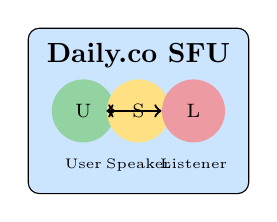
\begin{tikzpicture}[scale=0.7]
          % SFU
          \draw[fill=accent!20, rounded corners] (0,0) rectangle (4,3);
          \node at (2,2.5) {\textbf{Daily.co SFU}};

          % Participants
          \node[circle, fill=success!50, minimum size=0.8cm] (u) at (1,1.5) {\scriptsize U};
          \node[circle, fill=warning!50, minimum size=0.8cm] (s) at (2,1.5) {\scriptsize S};
          \node[circle, fill=danger!50, minimum size=0.8cm] (l) at (3,1.5) {\scriptsize L};

          % Labels
          \node[below] at (1,0.8) {\tiny User};
          \node[below] at (2,0.8) {\tiny Speaker};
          \node[below] at (3,0.8) {\tiny Listener};

          % Arrows
          \draw[<->, thick] (u) -- (s);
          \draw[->, thick] (u) -- (l);
        \end{tikzpicture}
      \end{center}

      \vspace{0.3cm}
      \textbf{3参加者構成}:
      \begin{itemize}
        \item User(ブラウザ)
        \item Vapi Speaker(応答)
        \item Vapi Listener(聞き取り)
      \end{itemize}
    \end{column}
  \end{columns}
\end{frame}

% ----- Section 3: Protocol -----
\section{プロトコル詳細}

\begin{frame}{通話開始シーケンス (概要)}
  \begin{center}
    \begin{tikzpicture}[scale=0.65, every node/.style={scale=0.65}]
      % Participants
      \node[draw, fill=light, minimum width=1.5cm] (user) at (0,6) {User};
      \node[draw, fill=success!20, minimum width=1.5cm] (widget) at (3,6) {Widget};
      \node[draw, fill=accent!20, minimum width=1.5cm] (clerk) at (6,6) {Clerk};
      \node[draw, fill=accent!20, minimum width=1.5cm] (vapi) at (9,6) {VAPI};
      \node[draw, fill=accent!20, minimum width=1.5cm] (daily) at (12,6) {Daily.co};

      % Lifelines
      \draw[dashed] (0,5.5) -- (0,0);
      \draw[dashed] (3,5.5) -- (3,0);
      \draw[dashed] (6,5.5) -- (6,0);
      \draw[dashed] (9,5.5) -- (9,0);
      \draw[dashed] (12,5.5) -- (12,0);

      % Messages
      \draw[->, thick] (0,5) -- (3,5) node[midway, above] {\scriptsize Click};
      \draw[->, thick] (3,4.5) -- (6,4.5) node[midway, above] {\scriptsize 認証};
      \draw[<-, thick] (3,4) -- (6,4);

      \draw[->, thick] (3,3.5) -- (9,3.5) node[midway, above] {\scriptsize POST /call/web};
      \draw[<-, thick] (3,3) -- (9,3) node[midway, above] {\scriptsize roomUrl};

      \draw[->, thick] (3,2.5) -- (12,2.5) node[midway, above] {\scriptsize WebSocket};
      \draw[<-, thick] (3,2) -- (12,2) node[midway, above] {\scriptsize sig-ack};

      \draw[->, thick] (3,1.5) -- (12,1.5) node[midway, above] {\scriptsize WebRTC};
      \draw[<->, thick, accent] (3,0.5) -- (12,0.5) node[midway, above] {\scriptsize 音声ストリーム};
    \end{tikzpicture}
  \end{center}
\end{frame}

\begin{frame}{プロトコルフェーズ}
  \begin{table}
    \centering
    \begin{tabular}{clp{7cm}}
      \toprule
      \textbf{\#} & \textbf{フェーズ} & \textbf{詳細} \\
      \midrule
      1 & 認証 & Clerk \texttt{POST /sessions/\{id\}/touch} \\
      2 & VAPI初期化 & \texttt{POST /call/web} + assistantId \\
      3 & Daily.co接続 & \texttt{POST /rooms/check/vapi/\{roomId\}} \\
      4 & WebSocket & SFUへ接続、\texttt{join-for-sig} \\
      5 & WebRTC & \texttt{create-transport}, \texttt{send-track} \\
      6 & エージェント参加 & Vapi Speaker/Listener が \texttt{sig-presence} \\
      7 & 音声会話 & RTPパケット双方向ストリーミング \\
      8 & トークン更新 & 45秒ごとにClerk JWT更新 \\
      \bottomrule
    \end{tabular}
  \end{table}
\end{frame}

\begin{frame}[fragile]{WebRTC詳細}
  \begin{columns}
    \begin{column}{0.5\textwidth}
      \textbf{トランスポート設定}
      \begin{itemize}
        \item 送信 (send) + 受信 (recv)
        \item ICE: Cloudflare STUN, Twilio TURN
        \item DTLS暗号化
      \end{itemize}

      \vspace{0.5cm}
      \textbf{音声トラック}
      \begin{itemize}
        \item コーデック: Opus 48kHz
        \item メディアタグ: \texttt{cam-audio}
        \item SSRC割り当て
      \end{itemize}
    \end{column}
    \begin{column}{0.5\textwidth}
      \begin{block}{send-track メッセージ}
        \begin{lstlisting}
{
  "transportId": "427...",
  "kind": "audio",
  "rtpParameters": {
    "codecs": [{
      "mimeType": "opus",
      "clockRate": 48000
    }]
  }
}
        \end{lstlisting}
      \end{block}
    \end{column}
  \end{columns}
\end{frame}

% ----- Section 4: Unique Value -----
\section{独自開発部分}

\begin{frame}{独自開発 vs 外部依存}
  \begin{center}
    \begin{tikzpicture}
      % Axes
      \draw[->] (0,0) -- (8,0) node[right] {差別化};
      \draw[->] (0,0) -- (0,5) node[above] {独自性};

      % Quadrant labels
      \node[secondary] at (2,4.5) {\scriptsize 高独自・低差別化};
      \node[secondary] at (6,4.5) {\scriptsize 高独自・高差別化};
      \node[secondary] at (2,0.5) {\scriptsize 低独自・低差別化};
      \node[secondary] at (6,0.5) {\scriptsize 低独自・高差別化};

      % Grid
      \draw[dashed, secondary] (4,0) -- (4,5);
      \draw[dashed, secondary] (0,2.5) -- (8,2.5);

      % Items
      \node[circle, fill=success, text=white, minimum size=0.8cm] at (6.5,4) {\scriptsize 1};
      \node[circle, fill=success, text=white, minimum size=0.8cm] at (5.5,3.5) {\scriptsize 2};
      \node[circle, fill=warning, minimum size=0.8cm] at (6,1.5) {\scriptsize 3};
      \node[circle, fill=danger, text=white, minimum size=0.8cm] at (2,1) {\scriptsize 4};

      % Legend
      \node[right] at (9,4) {\scriptsize 1: プロンプト設計};
      \node[right] at (9,3.5) {\scriptsize 2: Widget UI};
      \node[right] at (9,1.5) {\scriptsize 3: Backend API};
      \node[right] at (9,1) {\scriptsize 4: 音声AI基盤};
    \end{tikzpicture}
  \end{center}
\end{frame}

\begin{frame}{独自開発コンポーネント}
  \begin{columns}
    \begin{column}{0.5\textwidth}
      \textbf{1. プロンプト設計} \textcolor{success}{\faCheckCircle}
      \begin{itemize}
        \item EC販売特化シナリオ
        \item 商品コンテキスト注入
        \item 日本語最適化
      \end{itemize}

      \vspace{0.3cm}
      \textbf{2. Widget UI} \textcolor{success}{\faCheckCircle}
      \begin{itemize}
        \item ブランドカスタマイズ
        \item 商品ページ連携
        \item カートUI統合
      \end{itemize}
    \end{column}
    \begin{column}{0.5\textwidth}
      \textbf{3. Backend API} \textcolor{success}{\faCheckCircle}
      \begin{itemize}
        \item 13 Function Tools
        \item 商品/カート/注文API
        \item ナレッジベース
      \end{itemize}

      \vspace{0.3cm}
      \textbf{4. 音声AI基盤} \textcolor{danger}{\faTimesCircle}
      \begin{itemize}
        \item VAPI完全依存
        \item カスタマイズ制限
        \item コスト課題
      \end{itemize}
    \end{column}
  \end{columns}
\end{frame}

% ----- Section 5: Competition -----
\section{競合分析}

\begin{frame}{競合マップ}
  \begin{center}
    \begin{tikzpicture}[scale=0.9]
      % Axes
      \draw[->] (0,0) -- (8,0) node[right] {カスタマイズ性};
      \draw[->] (0,0) -- (0,5) node[above] {汎用性};

      % Competitors
      \node[circle, fill=accent, text=white, minimum size=1cm] (vapi) at (3,4) {VAPI};
      \node[circle, fill=success, text=white, minimum size=1cm] (pipecat) at (7,4) {Pipecat};
      \node[circle, fill=warning, minimum size=1cm] (retell) at (2,1.5) {Retell};
      \node[circle, fill=danger, text=white, minimum size=1cm] (omakase) at (5,1.5) {omakase};
      \node[circle, fill=secondary, text=white, minimum size=1cm] (repai) at (6,2) {Rep AI};

      % Labels
      \node[below] at (vapi) {\scriptsize 汎用API};
      \node[below] at (pipecat) {\scriptsize OSS};
      \node[below] at (retell) {\scriptsize 電話特化};
      \node[below] at (omakase) {\scriptsize EC特化};
      \node[below] at (repai) {\scriptsize EC};
    \end{tikzpicture}
  \end{center}

  \vspace{0.3cm}
  \textbf{omakase.ai のポジション}: EC特化 × 日本市場 × 音声AI
\end{frame}

\begin{frame}{機能比較}
  \begin{table}
    \centering
    \begin{tabular}{lccccc}
      \toprule
      \textbf{機能} & \textbf{omakase} & \textbf{VAPI} & \textbf{Pipecat} & \textbf{Rep AI} & \textbf{Retell} \\
      \midrule
      音声対話 & \textcolor{success}{\faCheck} & \textcolor{success}{\faCheck} & \textcolor{success}{\faCheck} & \textcolor{success}{\faCheck} & \textcolor{success}{\faCheck} \\
      Webウィジェット & \textcolor{success}{\faCheck} & \textcolor{success}{\faCheck} & \textcolor{warning}{\faMinus} & \textcolor{success}{\faCheck} & \textcolor{danger}{\faTimes} \\
      EC特化 & \textcolor{success}{\faCheck} & \textcolor{danger}{\faTimes} & \textcolor{danger}{\faTimes} & \textcolor{success}{\faCheck} & \textcolor{danger}{\faTimes} \\
      日本語 & \textcolor{success}{\faCheck} & \textcolor{success}{\faCheck} & \textcolor{success}{\faCheck} & \textcolor{warning}{\faQuestion} & \textcolor{success}{\faCheck} \\
      カート統合 & \textcolor{success}{\faCheck} & \textcolor{warning}{\faMinus} & \textcolor{warning}{\faMinus} & \textcolor{success}{\faCheck} & \textcolor{danger}{\faTimes} \\
      OSS & \textcolor{danger}{\faTimes} & \textcolor{danger}{\faTimes} & \textcolor{success}{\faCheck} & \textcolor{danger}{\faTimes} & \textcolor{danger}{\faTimes} \\
      \bottomrule
    \end{tabular}
  \end{table}
\end{frame}

% ----- Section 6: Proposal -----
\section{改善提案}

\begin{frame}{課題と改善策}
  \begin{columns}
    \begin{column}{0.5\textwidth}
      \textbf{現状の課題}
      \begin{enumerate}
        \item \textcolor{danger}{\faExclamationTriangle} VAPI完全依存
        \item \textcolor{danger}{\faExclamationTriangle} コスト構造
        \item \textcolor{warning}{\faExclamationCircle} カスタマイズ制限
        \item \textcolor{warning}{\faExclamationCircle} ベンダーロックイン
      \end{enumerate}
    \end{column}
    \begin{column}{0.5\textwidth}
      \textbf{改善策: Pipecat移行}
      \begin{enumerate}
        \item \textcolor{success}{\faCheck} 自社管理の音声AI
        \item \textcolor{success}{\faCheck} コスト50\%削減
        \item \textcolor{success}{\faCheck} 完全カスタマイズ
        \item \textcolor{success}{\faCheck} マルチベンダー対応
      \end{enumerate}
    \end{column}
  \end{columns}

  \vspace{0.5cm}

  \begin{center}
    \begin{tikzpicture}
      \node[draw, fill=danger!20, rounded corners] (before) at (0,0) {VAPI依存};
      \node[draw, fill=success!20, rounded corners] (after) at (6,0) {Pipecat自社管理};
      \draw[->, very thick, accent] (before) -- (after) node[midway, above] {移行};
    \end{tikzpicture}
  \end{center}
\end{frame}

\begin{frame}{Pipecat移行計画}
  \begin{center}
    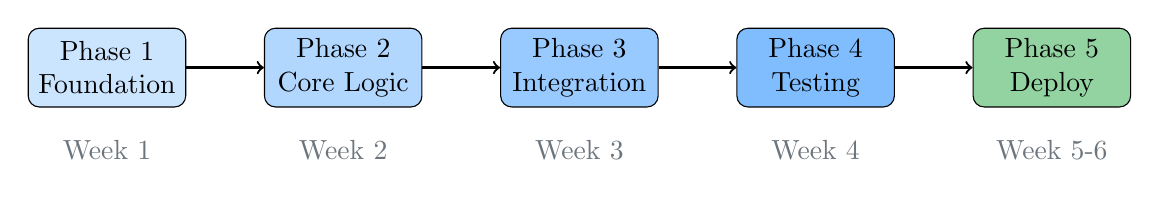
\begin{tikzpicture}[
      phase/.style={draw, rounded corners, minimum width=2cm, minimum height=1cm, align=center}
    ]
      % Phases
      \node[phase, fill=accent!20] (p1) at (0,0) {Phase 1\\Foundation};
      \node[phase, fill=accent!30] (p2) at (3,0) {Phase 2\\Core Logic};
      \node[phase, fill=accent!40] (p3) at (6,0) {Phase 3\\Integration};
      \node[phase, fill=accent!50] (p4) at (9,0) {Phase 4\\Testing};
      \node[phase, fill=success!50] (p5) at (12,0) {Phase 5\\Deploy};

      % Arrows
      \draw[->, thick] (p1) -- (p2);
      \draw[->, thick] (p2) -- (p3);
      \draw[->, thick] (p3) -- (p4);
      \draw[->, thick] (p4) -- (p5);

      % Timeline
      \node[below, secondary] at (0,-0.8) {Week 1};
      \node[below, secondary] at (3,-0.8) {Week 2};
      \node[below, secondary] at (6,-0.8) {Week 3};
      \node[below, secondary] at (9,-0.8) {Week 4};
      \node[below, secondary] at (12,-0.8) {Week 5-6};
    \end{tikzpicture}
  \end{center}

  \vspace{0.5cm}

  \begin{table}
    \centering
    \begin{tabular}{lll}
      \toprule
      \textbf{Phase} & \textbf{内容} & \textbf{成果物} \\
      \midrule
      1 & Pipecat基本パイプライン & PoC動作確認 \\
      2 & Function Tools + Backend連携 & 13ツール動作 \\
      3 & Widget統合 + Feature Flag & 切り替え可能 \\
      4 & 負荷テスト + 最適化 & <600msレイテンシ \\
      5 & Staging → Production & 本番稼働 \\
      \bottomrule
    \end{tabular}
  \end{table}
\end{frame}

\begin{frame}{期待効果}
  \begin{columns}
    \begin{column}{0.5\textwidth}
      \begin{block}{\faChartLine\ コスト削減}
        \begin{itemize}
          \item VAPI料金: \textcolor{danger}{-100\%}
          \item 新規コスト: Deepgram + ElevenLabs
          \item \textbf{純削減: 30-50\%}
        \end{itemize}
      \end{block}

      \begin{block}{\faRocket\ パフォーマンス}
        \begin{itemize}
          \item レイテンシ: 800ms → \textbf{<600ms}
          \item 中間サービス削減
        \end{itemize}
      \end{block}
    \end{column}
    \begin{column}{0.5\textwidth}
      \begin{block}{\faCogs\ カスタマイズ}
        \begin{itemize}
          \item プロンプト完全制御
          \item STT/TTS選択自由
          \item 独自機能追加可能
        \end{itemize}
      \end{block}

      \begin{block}{\faShield*\ リスク軽減}
        \begin{itemize}
          \item ベンダーロックイン解消
          \item 障害時の切り替え可能
        \end{itemize}
      \end{block}
    \end{column}
  \end{columns}
\end{frame}

% ----- Summary -----
\section{まとめ}

\begin{frame}{まとめ}
  \begin{enumerate}
    \item \textbf{現状分析}: VAPI/Daily.coに高度依存、独自価値はUI/プロンプト
    \item \textbf{プロトコル}: HAR解析で詳細フロー特定完了
    \item \textbf{競合}: EC特化×日本市場でのニッチポジション
    \item \textbf{提案}: Pipecat移行でコスト削減・カスタマイズ強化
  \end{enumerate}

  \vspace{0.5cm}

  \begin{block}{Next Steps}
    \begin{enumerate}
      \item Pipecat PoC実施 (Week 1)
      \item コスト比較・検証
      \item 移行判断
    \end{enumerate}
  \end{block}
\end{frame}

\begin{frame}{}
  \begin{center}
    \vspace{2cm}
    {\Huge\textbf{Thank You}}

    \vspace{1cm}

    {\large Questions?}

    \vspace{2cm}

    {\small\textcolor{secondary}{Confidential - Internal Use Only}}
  \end{center}
\end{frame}

% ----- Appendix -----
\appendix

\begin{frame}{Appendix: プロトコルシーケンス図}
  \begin{center}
    \includegraphics[width=0.95\textwidth]{images/protocol.png}
  \end{center}
\end{frame}

\begin{frame}{Appendix: アーキテクチャ図}
  \begin{center}
    \includegraphics[width=0.9\textwidth]{images/omakase-ai-architecture.png}
  \end{center}
\end{frame}

\end{document}
